\documentclass[10pt,a4paper]{article}

% ── Encoding & fonts (XeLaTeX) ────────────────────────────────────────────
\usepackage{fontspec}
\setmainfont{Helvetica Neue}[
  UprightFont = Helvetica Neue Thin,
  BoldFont    = Helvetica Neue Medium,
  ItalicFont  = Helvetica Neue Thin Italic,
  Scale       = 1.0,
  AutoFakeBold,
  AutoFakeSlant=0.2,
]
\setmonofont{Menlo}[Scale=0.85]

% ── Layout ────────────────────────────────────────────────────────────────
\usepackage[a4paper,margin=1.6cm,bottom=1.8cm]{geometry}
\usepackage{microtype}
\usepackage{enumitem}
\setlist{nosep,leftmargin=*,topsep=2pt,partopsep=0pt,itemsep=2pt}
\usepackage{xcolor}
\definecolor{nileblue}{RGB}{30, 90, 150}
\definecolor{nilegray}{RGB}{120, 120, 130}
\definecolor{rowblue}{RGB}{235, 242, 250}
\definecolor{boxbg}{RGB}{245, 247, 252}
\definecolor{boxborder}{RGB}{200, 215, 235}
\definecolor{ruleline}{RGB}{200, 210, 220}

% ── Section formatting ────────────────────────────────────────────────────
\usepackage[explicit]{titlesec}
\titleformat{\section}{\normalfont\Large\bfseries\color{nileblue}}{\thesection.}{0.5em}{#1}[\vspace{-4pt}\noindent\textcolor{ruleline}{\rule{\linewidth}{0.5pt}}]
\titleformat{\subsection}{\normalfont\large\bfseries}{\thesubsection}{0.5em}{#1}
\titlespacing*{\section}{0pt}{0.9em}{0.45em}
\titlespacing*{\subsection}{0pt}{0.55em}{0.2em}

% ── Tables ────────────────────────────────────────────────────────────────
\usepackage{booktabs}
\usepackage{tabularx}
\usepackage{array}
\usepackage{colortbl}
\renewcommand{\arraystretch}{1.15}
\newcolumntype{L}[1]{>{\raggedright\arraybackslash}p{#1}}

% ── Diagrams ──────────────────────────────────────────────────────────────
\usepackage{tikz}
\usetikzlibrary{positioning,shapes.geometric,arrows.meta,backgrounds,fit,calc}

\tikzset{
  agbox/.style={
    rectangle, rounded corners=4pt, draw=nileblue, line width=0.6pt,
    fill=boxbg, align=center,
    minimum height=1.0cm, minimum width=2.4cm,
    inner sep=4pt, font=\small
  },
  toolbox/.style={
    agbox, fill=white, draw=nilegray, font=\footnotesize
  },
  terminal/.style={
    agbox, fill=nileblue!10, draw=nileblue, font=\small\bfseries
  },
  decision/.style={
    diamond, draw=nileblue, line width=0.6pt, fill=white,
    aspect=2, inner sep=2pt, font=\footnotesize
  },
  arrow/.style={-{Stealth[scale=1.1]}, line width=0.55pt, draw=nilegray},
  labeledge/.style={font=\footnotesize\itshape, fill=white, inner sep=1pt},
  phasebox/.style={
    rectangle, rounded corners=8pt, draw=nileblue!40, line width=0.5pt,
    dashed, inner sep=12pt
  },
}

% ── Inline code ───────────────────────────────────────────────────────────
\usepackage{soul}
\sethlcolor{boxbg}
\newcommand{\code}[1]{\colorbox{boxbg}{\strut\texttt{\small #1}}}

% ── Hyperlinks ────────────────────────────────────────────────────────────
\usepackage[hidelinks]{hyperref}

% ── Caption ───────────────────────────────────────────────────────────────
\usepackage{caption}
\captionsetup{font={small,it},labelfont=bf,labelsep=endash}

\pagenumbering{gobble}

\begin{document}

% ── Title block ───────────────────────────────────────────────────────────
\begingroup
\setlength{\parindent}{0pt}
{\Huge\bfseries\color{nileblue} Multi-Agent Legal Explainer\par}
\vspace{2pt}
{\large\color{nilegray} A LangGraph-orchestrated agent over the Egyptian Civil Code\par}
\vspace{6pt}
\textcolor{ruleline}{\rule{\linewidth}{0.6pt}}\par\vspace{4pt}
{\small\color{nilegray}\itshape Technical Report \quad\textbullet\quad \textbf{Stack:} Claude Agent SDK \textbullet{} LangGraph \textbullet{} LightRAG knowledge graph \textbullet{} Ollama Qwen3 embeddings \textbullet{} NLTK Punkt \textbullet{} Gradio UI\par}
\textcolor{ruleline}{\rule{\linewidth}{0.6pt}}
\endgroup

\vspace{6pt}

% ── 1. Overview ───────────────────────────────────────────────────────────
\section{Overview \& Objective}

The system answers natural-language legal questions about the Egyptian Civil Code by orchestrating \textbf{three specialised Claude subagents} behind a \textbf{LangGraph} state machine. An LLM-based \textit{router} classifies each query as \emph{simple}, \emph{medium}, or \emph{complex} and dispatches it down the cheapest path that yields a correct, grounded answer. Tools replace recall with lookup: a curated bilingual glossary, a deterministic article-keyed statute index, a graph-RAG retriever, and an optional web search. Every claim is cited; the system refuses rather than hallucinates.

The package implements the two product epics targeted in this work:
\begin{itemize}
\item \textbf{Epic 6 — Tooling \& Function Calling.} Strict-schema tools registered as a single MCP server, so the model reaches for a deterministic function instead of guessing definitions or article text.
\item \textbf{Epic 7 — Multi-Agent Collaboration.} A baseline two-role pipeline (\emph{Researcher} \(\rightarrow\) \emph{Explainer}) is shipped alongside the orchestrated flow, and a parallel eval harness compares the two on the same 424-case RAFT validation set.
\end{itemize}

% ── 2. System Architecture ────────────────────────────────────────────────
\section{System Architecture}

The orchestrator is a LangGraph state machine. Each node is an async function that mutates a shared \code{GraphState}; conditional edges route between nodes based on the router's decision. Subagents are themselves wrapped \code{query()} calls to Claude, each with its own system prompt and tool allow-list — they are the \emph{nodes} of the graph, not orchestrators.

\begin{center}
\resizebox{\linewidth}{!}{%
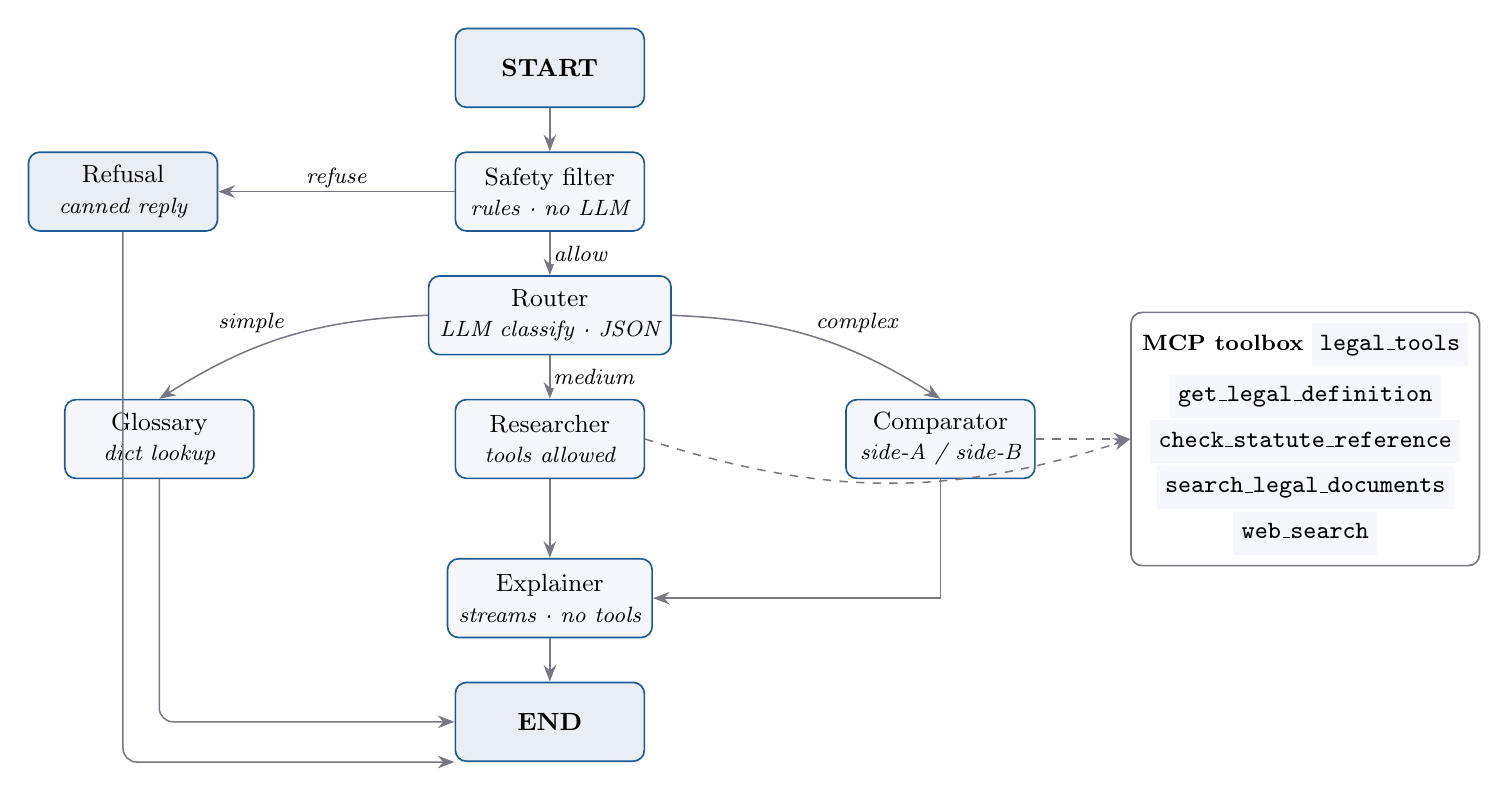
\begin{tikzpicture}[node distance=0.55cm and 0.8cm]

  \node[terminal] (start) {START};
  \node[agbox, below=of start] (safety) {Safety filter\\\footnotesize\itshape rules · no LLM};
  \node[agbox, below=of safety] (router) {Router\\\footnotesize\itshape LLM classify · JSON};

  \node[agbox, below left=of router, xshift=-1.4cm] (gloss) {Glossary\\\footnotesize\itshape dict lookup};
  \node[agbox, below=of router] (researcher) {Researcher\\\footnotesize\itshape tools allowed};
  \node[agbox, below right=of router, xshift=1.4cm] (comparator) {Comparator\\\footnotesize\itshape side-A / side-B};

  \node[agbox, below=1.0cm of researcher] (explainer) {Explainer\\\footnotesize\itshape streams · no tools};

  \node[agbox, fill=nileblue!10, left=3.0cm of safety] (refusal) {Refusal\\\footnotesize\itshape canned reply};
  \node[terminal, below=of explainer] (endnode) {END};

  \draw[arrow] (start) -- (safety);
  \draw[arrow] (safety) -- node[labeledge,right]{allow} (router);
  \draw[arrow] (safety) -- node[labeledge,above]{refuse} (refusal);

  % Refusal routes down its own column past Glossary, then right into END's
  % south-west corner — keeps it clear of Glossary's exit line.
  \draw[arrow, rounded corners=5pt]
    (refusal.south) -- (refusal.south |- endnode.south)
    -- (endnode.south west);

  \draw[arrow] (router.west) to[bend right=15] node[labeledge,above left]{simple} (gloss.north);
  \draw[arrow] (router) -- node[labeledge,right]{medium} (researcher);
  \draw[arrow] (router.east) to[bend left=15] node[labeledge,above right]{complex} (comparator.north);

  % Glossary takes the direct middle-left path into END's west side.
  \draw[arrow, rounded corners=5pt] (gloss.south) |- (endnode.west);
  \draw[arrow] (researcher) -- (explainer);
  \draw[arrow] (comparator.south) |- (explainer.east);
  \draw[arrow] (explainer) -- (endnode);

  % MCP toolbox sits to the right of Comparator so it doesn't collide with it.
  \node[toolbox, right=1.2cm of comparator] (tools) {\textbf{MCP toolbox} \code{legal\_tools}\\[2pt]
    \footnotesize\code{get\_legal\_definition}\\
    \footnotesize\code{check\_statute\_reference}\\
    \footnotesize\code{search\_legal\_documents}\\
    \footnotesize\code{web\_search}};
  % Researcher reaches over Comparator to the toolbox (curve to avoid overlap).
  \draw[arrow, dashed] (researcher.east) to[bend right=18] (tools.west);
  \draw[arrow, dashed] (comparator.east) -- (tools.west);

\end{tikzpicture}%
}
\end{center}

\captionsetup{type=figure}
\captionof{figure}{Compiled LangGraph orchestrator. Bold boxes are terminal nodes (START, END, refusal); rounded boxes are agent or tool nodes. Dashed arrows show MCP tool access — only Researcher and Comparator may call tools; Explainer never does (it grounds strictly on the JSON it receives from the previous node).}

% ── 3. Subagents & Models ─────────────────────────────────────────────────
\section{Subagents \& Models}

\begin{tabularx}{\linewidth}{l l X}
\toprule
\textbf{Role} & \textbf{Model} & \textbf{Why this choice} \\
\midrule
\rowcolor{rowblue}
Orchestrator (LangGraph state machine) & deterministic Python & No LLM in the control plane; pure flow logic + edge predicates compiled once. \\
Router & Claude (single classify call) & One short prompt \(\rightarrow\) JSON \{complexity, glossary\_term\_id, reason\}; defensively validated against the glossary so a hallucinated id downgrades to medium. \\
\rowcolor{rowblue}
Researcher (T≈0.2) & Claude with MCP tools & Retrieves and extracts; emits structured JSON (\code{key\_passages}, \code{key\_facts}, \code{ambiguities}). Never synthesizes. \\
Comparator (T≈0.3) & Claude with MCP tools & Two-sided structured output (\code{side\_a}, \code{side\_b}, \code{shared\_ground}, \code{differences}); prompt forces side-isolated retrieval. \\
\rowcolor{rowblue}
Explainer (T≈0.4) & Claude, no tools & Receives structured findings, writes the user-facing answer; mandatory disclaimer; language matches the user query. Streams chunks for live UI. \\
\bottomrule
\end{tabularx}

\smallskip
\noindent\textit{The three subagents share the same MCP toolbox but with different allow-lists. The Explainer is intentionally toolless: its only grounding is the JSON the previous subagent produced, which structurally prevents it from inventing facts.}

% ── 4. Methodology — Tool Catalog ─────────────────────────────────────────
\section{Methodology — Tool Catalog (Epic 6)}

Tools are bundled into one MCP server (\code{legal\_tools}) via the Claude Agent SDK's \code{create\_sdk\_mcp\_server}; each subagent registers it and exposes only the subset it is permitted to call. Tool descriptions tell the model \emph{when to call and when not to}, keeping the catalog small and high-signal.

\begin{tabularx}{\linewidth}{>{\raggedright\arraybackslash}p{3.6cm} X >{\small\raggedright\arraybackslash}p{4.0cm}}
\toprule
\textbf{Tool} & \textbf{What it does} & \textbf{Backing store} \\
\midrule
\code{get\_legal\_definition} & Bilingual EN/AR glossary of 15 curated civil-law terms with cross-language aliases (\emph{indemnity}, \emph{compensation}, and the Arabic equivalents all resolve to one canonical entry). & \code{data/glossary.json} \\
\rowcolor{rowblue}
\code{check\_statute\_reference} & Parses citations in \emph{Article~N} or \emph{Art.~N} format (English and Arabic accepted) and returns the verbatim article text. Returns \{found:\,false\} on miss rather than fabricating. & \code{articles\_index.json} (2{,}164 articles, parsed once from EgyptianLaw.pdf) \\
\code{search\_legal\_documents} & Graph-RAG retrieval over the Egyptian Civil Code knowledge graph. Returns structured entities, relationships, and source chunks; \textbf{never invokes its own LLM} for synthesis or keyword extraction (see §6). & LightRAG \code{aquery\_data()} \\
\rowcolor{rowblue}
\code{web\_search} & DuckDuckGo wrapper for current-events / recent-amendment questions outside the static corpus. & \code{ddgs} package \\
\bottomrule
\end{tabularx}

\smallskip
\noindent\textbf{Failure mode discipline.} Every tool returns a structured \{found:\,false, reason:\,…\} or \{ok:\,false, message:\,…\} on a miss, never an exception. The model is instructed to honour these and surface them to the user, which is the difference between an honest ``I don't have Article 1341'' and a confidently wrong answer.

% ── 5. Methodology — Orchestration ────────────────────────────────────────
\section{Methodology — Orchestration (Epic 7)}

\subsection{The LLM Router}
A single Claude classification call replaces the brittle keyword regex of v1. The router prompt embeds the 15 canonical glossary ids inline so the model knows what \emph{simple} actually means, and asks for strict JSON:

\smallskip
\colorbox{boxbg}{\parbox{0.96\linewidth}{\small\ttfamily
\{"complexity": "simple|medium|complex",\\
\hphantom{X}"glossary\_term\_id": "<id or null>",\\
\hphantom{X}"reason": "<one short sentence>"\}
}}

\smallskip
\noindent The Python side defensively verifies that any \code{glossary\_term\_id} actually exists in the glossary; otherwise it downgrades to \emph{medium}. This eliminates a class of bugs (an LLM-hallucinated id leading to a nonsense glossary lookup) that occurred in the v1 rule-based router.

\subsection{Path Dispatch}
\begin{tabularx}{\linewidth}{l X l l}
\toprule
\textbf{Path} & \textbf{When chosen} & \textbf{LLM calls} & \textbf{Typical latency} \\
\midrule
\rowcolor{rowblue}
\code{simple} & Router identifies a single glossary term & 1 (router) & $\sim$1 s \\
\code{medium} & Article reference or single-topic query & 3 (router + Researcher + Explainer) & $\sim$50 s \\
\rowcolor{rowblue}
\code{complex} & Comparison / contrast keywords detected & 3 (router + Comparator + Explainer) & $\sim$70 s \\
\code{refused} & Safety filter matched off-policy patterns (case-advice, document drafting, out-of-jurisdiction) & \textbf{0} & $\sim$0 s \\
\bottomrule
\end{tabularx}

\subsection{State \& Observability}
\code{GraphState} is a \code{TypedDict} that each node enriches via partial updates — cost and duration accumulate as nodes return. A \code{FlowLogger} captures every event (safety verdict, router decision, subagent start/end, tool call, tool result, streaming answer chunks) into both an in-memory list (for the live UI) and a JSONL trace file at \code{reports/agent\_traces/}. The same logger is read by the Gradio app to render the live ``thinking'' panel and stream the answer token-by-token.

% ── 6. Knowledge Base (brief) ─────────────────────────────────────────────
\section{Knowledge Base (brief)}

Retrieval is secondary to this report, but the agent's grounding depends on it, so a one-paragraph summary: \textbf{EgyptianLaw.pdf} is parsed once with PyMuPDF, then \textbf{LightRAG} chunks ($\sim$4{,}000-token chunks with 200-token overlap), embeds each chunk with \textbf{Ollama Qwen3-Embedding 0.6B} (1024-dim, multilingual), and builds an entity/relation knowledge graph backed by NanoVectorDB. The result: 2{,}164 articles indexed, 1{,}285 entities, 1{,}474 relations. A separate deterministic pass produces \code{articles\_index.json} (article-keyed verbatim text) used by \code{check\_statute\_reference} for citation-grade lookups.

\smallskip
\noindent\textbf{No-LLM retrieval invariant.} The \code{search\_legal\_documents} tool calls LightRAG's \code{aquery\_data()} with pre-extracted \code{hl\_keywords} and \code{ll\_keywords} computed by NLTK Punkt + bilingual stopwords + glossary/article-ref matching, which makes LightRAG bypass its internal LLM-based extractor entirely. A defensive \code{\_llm\_guard} callback raises if any code path tries to invoke an LLM inside the retrieval — so we cannot silently burn tokens during tool use.

% ── 7. Evaluation ─────────────────────────────────────────────────────────
\section{Evaluation}

The eval harness runs the orchestrator (or the baseline two-role pipeline) against the existing repo's RAFT validation set (\code{qa\_pairs\_raft\_val.jsonl}, 424 bilingual cases). It is asyncio-parallel by default with crash-safe streaming JSONL output, and computes one metric absent from the original judge harness: \textbf{retrieval\_hit@k} — does the prediction cite the dataset's gold \code{article\_key}?

\begin{tabularx}{\linewidth}{l X}
\toprule
\textbf{Stage} & \textbf{Technique / output} \\
\midrule
\rowcolor{rowblue}
Generation & \code{run\_orchestrated\_lg(query)} or \code{run\_baseline(query)} per case; parallel via \code{asyncio.Semaphore(N)} \\
Retrieval correctness & Regex on the gold \code{article\_key} — \emph{Article~N} (or its Arabic equivalent) present in the prediction \\
\rowcolor{rowblue}
Quality scoring & Delegated to the repo's existing Claude-judge harness (\code{scripts/closed\_book\_recall\_eval.py}, 5-dim rubric: legal accuracy, completeness, house style, language, faithfulness) \\
Latency / cost & Per-case \code{duration\_ms} and \code{total\_cost\_usd} from each \code{OrchestratorResult}; p50/p90 in summary \\
\rowcolor{rowblue}
Path attribution & Tracks which orchestrator path served each case (simple/medium/complex/refused) for routing-effectiveness analysis \\
\bottomrule
\end{tabularx}

\smallskip
\noindent A \code{snapshot.py} script reads the streaming \code{.jsonl.partial} file mid-run, so a long sweep can be monitored live without disrupting it. The companion \code{compare\_baseline.py} prints a side-by-side latency / cost / hit-rate / path-distribution table between two prediction files.

% ── 8. Interface — Gradio app ─────────────────────────────────────────────
\section{Interface — Gradio App}

A Gradio UI (\code{gradio\_app.py}) lets a user type a question and observe the agent in real time. Three live panes update as the run progresses:

\begin{itemize}
\item \textbf{Answer} — the Explainer's final answer streams chunk-by-chunk (the SDK's \code{TextBlock}s feed a callback that appends to \code{FlowLogger.answer\_text}; the UI polls every 400 ms). A \code{▍} sentinel renders as a cursor while streaming.
\item \textbf{Thinking} — a collapsible accordion shows every flow event as it happens: query, safety verdict, router decision (including the LLM's reasoning), subagent start / end with cost and duration, every tool call with its arguments, every tool result with a one-line summary.
\item \textbf{Run metrics} — live aggregate: elapsed time, current path, tools called, tool call count, subagents active.
\end{itemize}

\noindent Pressing Enter in the prompt textbox submits the query. Six pre-built example queries demonstrate each path (simple glossary, medium English, medium Arabic, complex comparison, safety refusal). The interface is intentionally theme-aware via Gradio's CSS variables so it renders correctly in both light and dark mode.

% ── 9. Implementation notes ───────────────────────────────────────────────
\section{Key Implementation Notes}

\begin{itemize}
\item \textbf{Two engines side-by-side.} A legacy rule-based orchestrator (v1, \code{orchestrator.py}) is preserved for regression; the LangGraph + LLM-router orchestrator (v2, \code{orchestrator\_langgraph.py}) is the default. The eval runner picks via \code{--engine \{langgraph,legacy\}}, and both produce predictions in an identical JSON shape so the Claude-judge harness scores them unchanged.
\item \textbf{No mid-orchestration LLM in the retrieval path.} LightRAG normally calls an LLM for query-time keyword extraction; we pre-compute \code{hl\_keywords} and \code{ll\_keywords} deterministically and pass them on \code{QueryParam}, then guard with a callback that errors loudly if LightRAG still tries. This makes the tool's cost predictable.
\item \textbf{Structured failure beats fabrication.} Every tool returns \{found:\,false, reason:\,…\} for misses. The system prompts tell each subagent to honour these — so a question about an article outside the corpus produces an honest ``I don't have Article 1341'' instead of an invented one.
\item \textbf{Bilingual by design.} The glossary, the statute-citation parser, the keyword extractor, the safety patterns, the system prompts, and the disclaimer template are all dual-language; the Explainer's prompt mandates ``respond in the user's language.''
\item \textbf{Crash-safe eval.} The parallel runner appends every completed prediction to a \code{.jsonl.partial} file before the final \code{.json} is written, so a 7-hour run that crashes at case 220/424 still has 220 usable predictions on disk.
\end{itemize}

\smallskip
\noindent\colorbox{boxbg}{\parbox{0.96\linewidth}{\textbf{End-to-end at a glance:} \texttt{query \(\rightarrow\) safety \(\rightarrow\) LLM router \(\rightarrow\) \{glossary | Researcher | Comparator\} \(\rightarrow\) Explainer (streams) \(\rightarrow\) cited answer + disclaimer}}}

\end{document}
